\documentclass{../../slides-style}

\slidetitleext{Лекция 9: Качество программного обеспечения}{18.04.2023}{Качество ПО}

\begin{document}

    \begin{frame}[plain]
        \titlepage
    \end{frame}

    \section{Понятие качества ПО}

    \begin{frame}
        \frametitle{Что такое качество ПО?}
        \begin{itemize}
            \item Обывательский подход
            \begin{itemize}
                \item Лёгкость в использовании, производительность, отсутствие ошибок, документация, кроссплатформенность и т.п.
            \end{itemize}
            \item Профессиональный подход
            \begin{itemize}
                \item Соответствие требованиям (Crosby, 1979)
                \item Пригодность к использованию (Juran, Gryna, 1970)
            \end{itemize}
            \item Жизненный подход
            \begin{itemize}
                \item Соответствие всем требованиям, явным и неявным
            \end{itemize}
        \end{itemize}
    \end{frame}

    \begin{frame}
        \frametitle{Стоимость качества}
        \begin{itemize}
            \item Решения о качестве принимаются на этапе работы с требованиями
            \item Обычно заказчик полагает качество максимальным
            \item Стоимость:
            \begin{itemize}
                \item стоимость предупреждения дефектов (prevention cost)
                \item стоимость оценки (appraisal cost)
                \item стоимость внутренних сбоев (internal failure cost)
                \item стоимость внешних сбоев (external failure cost)
            \end{itemize}
        \end{itemize}
    \end{frame}

    \begin{frame}
        \begin{center}
            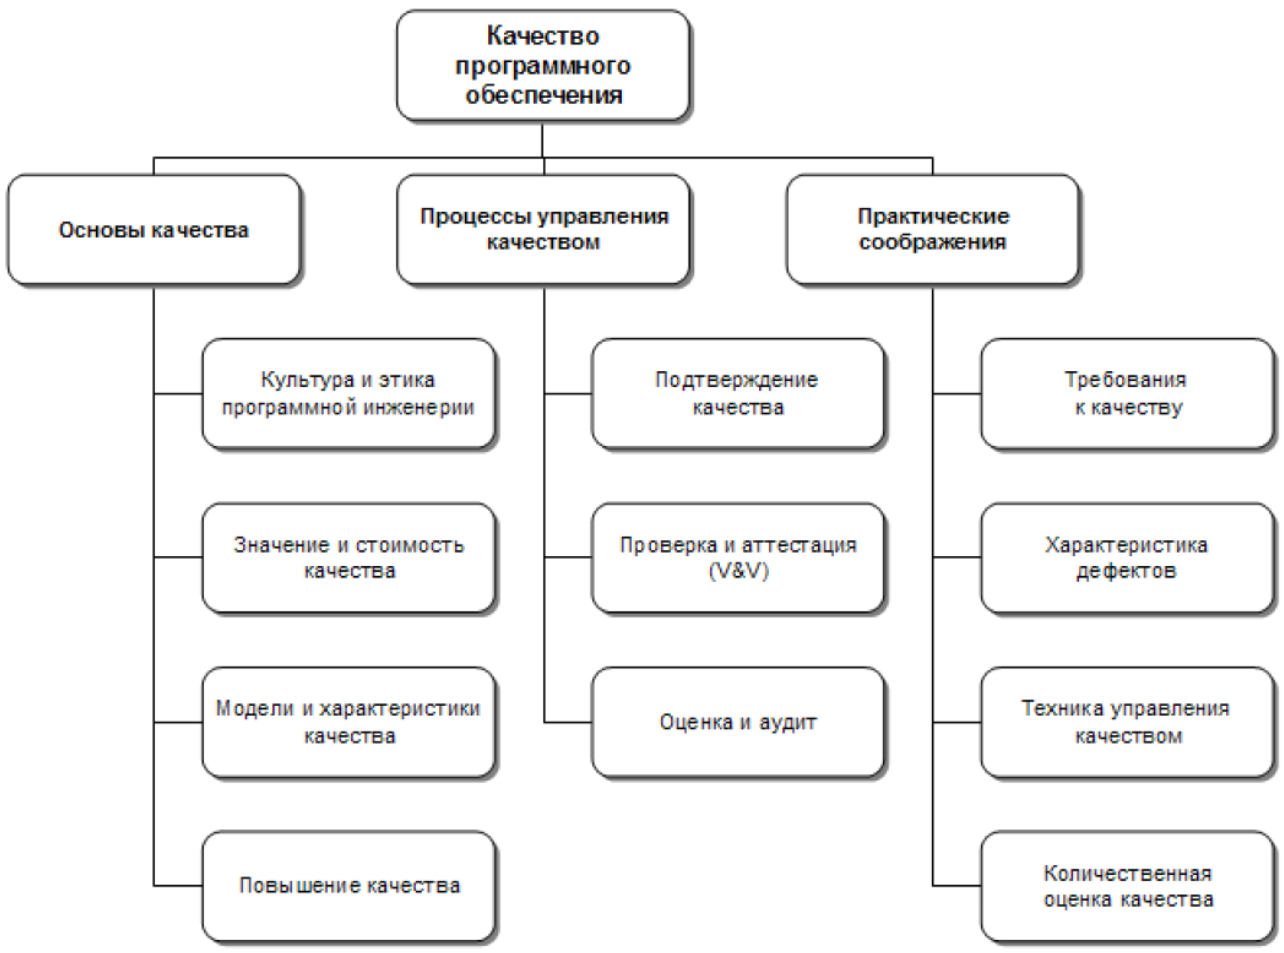
\includegraphics[width=0.9\textwidth]{quality.png}
        \end{center}
    \end{frame}

    \section{Модель качества ПО}

    \begin{frame}
        \frametitle{Модель качества ПО}
        \begin{itemize}
            \item Характеристики качества --- отдельные точки зрения пользователя на качество
            \item Атрибуты характеристик качества --- детализация разных аспектов характеристики
            \item Метрики качества
            \begin{itemize}
                \item Метод измерения атрибута
                \item Шкала измерения значений атрибута
                \item Вес (иногда)
            \end{itemize}
        \end{itemize}
    \end{frame}

    \subsection{Характеристики качества}

    \begin{frame}
        \frametitle{Характеристики качества ПО (ISO 25010:2011)}
        \begin{itemize}
            \item Функциональность
            \item Надежность
            \item Удобство использования
            \item Эффективность
            \item Сопровождаемость
            \item Переносимость
        \end{itemize}
    \end{frame}

    \begin{frame}
        \frametitle{Функциональность}
        \begin{itemize}
            \item Функциональная полнота (suitability)
            \item Правильность (точность) (accuracy)
            \item Функциональная совместимость (интероперабельность) (interoperability)
            \item Защищенность (security)
            \item Соответствие стандартам и правилам (compliance)
        \end{itemize}
    \end{frame}

    \begin{frame}
        \frametitle{Надежность}
        \begin{itemize}
            \item Безотказность (maturity)
            \item Устойчивость к отказам (fault tolerance)
            \item Восстанавливаемость (recoverability)
            \item Пригодноспособность (dependability)
            \begin{itemize}
                \item Готовность к использованию (availability)
                \item Готовностью к непрерывному функционированию (reliability)
                \item Безопасность для окружающей среды (safety)
                \item Секретность и сохранность информации (сonfidentiality)
                \item Устойчивость к самопроизвольному изменению (integrity)
                \item Простота выполнения операций обслуживания (maintainability)
            \end{itemize}
        \end{itemize}
    \end{frame}

    \begin{frame}
        \frametitle{Удобство использования}
        \begin{itemize}
            \item Понимаемость (understandability)
            \item Легкость изучения (learnability)
            \item Удобство работы (operability)
            \begin{itemize}
                \item Оперативность
                \item Согласованность
            \end{itemize}
            \item Привлекательность (attractiveness)
        \end{itemize}
    \end{frame}

    \begin{frame}
        \frametitle{Эффективность}
        \begin{itemize}
            \item Временная эффективность, реактивность (time behaviour)
            \item Эффективность ресурсов (resource utilisation)
        \end{itemize}
    \end{frame}

    \begin{frame}
        \frametitle{Сопровождаемость}
        \begin{itemize}
            \item Анализируемость (analyzability)
            \item Изменяемость (changeability)
            \item Стабильность (stability)
            \item Тестируемость (testability)
        \end{itemize}
    \end{frame}

    \begin{frame}
        \frametitle{Переносимость}
        \begin{itemize}
            \item Адаптивность (adaptability)
            \item Настраиваемость, простота инсталляции (installability)
            \item Сосуществование (coexistence)
            \item Заменяемость (replaceability)
        \end{itemize}
    \end{frame}

    \subsection{Метрики}

    \begin{frame}
        \frametitle{Метрики качества ПО}
        \begin{itemize}
            \item Функциональность: метрики тестирования
            \item Надежность: метрики тестирования, динамические метрики
            \item Удобство использования: метрики эргономики
            \item Эффективность: динамические метрики
            \item Сопровождаемость: метрики кода
            \item Переносимость: метрики кода
        \end{itemize}
    \end{frame}

    \begin{frame}
        \frametitle{Классификация метрик}
        \begin{itemize}
            \item Метрики программного продукта
            \begin{itemize}
                \item Внешние
                \begin{itemize}
                    \item Надежность
                    \item Функциональность
                    \item Сопровождение
                    \item Стоимость
                \end{itemize}
                \item Внутренние
                \begin{itemize}
                    \item Размер
                    \item Сложность
                    \item Стиль
                \end{itemize}
            \end{itemize}
            \item Метрики процесса
            \item Метрики использования
        \end{itemize}
    \end{frame}

    \begin{frame}
        \frametitle{Классификация метрик}
        \begin{itemize}
            \item Метрики программного продукта
            \item Метрики процесса
            \begin{itemize}
                \item Общее время разработки и отдельно время для каждой стадии
                \item Время модификации моделей
                \item Время выполнения работ на процессе
                \item Число найденных ошибок при инспектировании
                \item Стоимость проверки качества
                \item Стоимость процесса разработки
            \end{itemize}
            \item Метрики использования
        \end{itemize}
    \end{frame}

    \begin{frame}
        \frametitle{Классификация метрик}
        \begin{itemize}
            \item Метрики программного продукта
            \item Метрики процесса
            \item Метрики использования
            \begin{itemize}
                \item Точность и полнота реализации задач пользователя
                \item Затраченные ресурсы на эффективное решение задач пользователя
            \end{itemize}
        \end{itemize}
    \end{frame}

    \begin{frame}
        \frametitle{Что можно измерять?}
        \begin{itemize}
            \item Размер
            \begin{itemize}
                \item Число классов, строк в программе, объём памяти, ...
            \end{itemize}
            \item Переиспользуемость кода
            \begin{itemize}
                \item Переиспользуемые классы, наследуемые классы, зависимости, ...
            \end{itemize}
            \item Время
            \begin{itemize}
                \item Отклика, общего функционирования системы, выполнения компонента, ...
            \end{itemize}
            \item Усилия
            \begin{itemize}
                \item Производительность труда, трудоемкость, ...
            \end{itemize}
            \item Ошибки
            \begin{itemize}
                \item Количество ошибок, число отказов, ...
            \end{itemize}
        \end{itemize}
    \end{frame}

    \begin{frame}
        \frametitle{Простые метрики}
        \begin{itemize}
            \item Число строк кода (LOC/KLOC)
            \item Производительность = LOC / Затраты
            \item Удельная стоимость = Затраты / LOC
            \item Качество кода = Число ошибок / LOC
            \item Документированность = Число страниц документации / LOC
        \end{itemize}
    \end{frame}

    \begin{frame}
        \frametitle{Ещё метрики}
        \begin{itemize}
            \item Метрики Холстеда
            \item Метрики С. Чидамбера и К. Кемерера
            \item Метрики Ф. Абреу
            \item Метрики Л. Константейна и Э. Йордана
            \item Метрики Л. Отта и Б. Мехра
            \item Метрики Д. Биемена и Б. Кенга
            \item Метрики М. Лоренца и Д. Кидда
            \item Метрики Р. Байндера
            \item ...
        \end{itemize}
    \end{frame}

    \begin{frame}
        \frametitle{Метрики Холстеда}
        \begin{itemize}
            \item Number of Unique Operators (NUOprtr)
            \item Number of Unique Operands (NUOprnd)
            \item Number of Operators (Noprtr)
            \item Number of Operands (Noprnd)
            \item Halstead Program Volume (HPVol) $= (Noprtr + Noprnd) \times log_2(NUOprtr + NUOprnd)$
            \item Halstead Difficulty (HDiff) $= (\frac{NUOprtr}{2}) \times (\frac{Noprnd}{NUOprnd})$
            \item Halstead Effort (HEff) $= HDiff \times HPVol$
        \end{itemize}
    \end{frame}

    \begin{frame}
        \frametitle{Цикломатическая сложность}
        \begin{columns}
            \begin{column}{0.7\textwidth}
                \begin{itemize}
                    \item C $= E – N + 2P$
                    \item E --- число ребер
                    \item N --- число узлов
                    \item P --- число компонентов связности
                \end{itemize}
            \end{column}
            \begin{column}{0.3\textwidth}
                \begin{center}
                    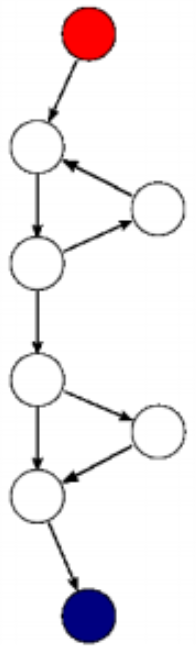
\includegraphics[height=0.8\textheight]{programGraph.png}
                \end{center}
            \end{column}
        \end{columns}
    \end{frame}

    \begin{frame}
        \frametitle{Метрики С. Чидамбера и К. Кемерера}
        \begin{itemize}
            \item Weighted Methods Per Class (WMC)
            \begin{itemize}
                \item $WMC = \sum_{i=1}^{n}C_i$, где $C_i$ --- как-то посчитанная сложность метода $i$
            \end{itemize}
            \item Depth of Inheritance Tree (DIT)
            \item Number of children (NOC)
            \item Coupling between object classes (СВО)
            \begin{itemize}
                \item Количество вызовов методов или полей
            \end{itemize}
            \item Response For a Class (RFC) $= |\{M\} \cup_{i} \{R_i\}| $
            \begin{itemize}
                \item $\{R_i\}$ --- множество методов, вызываемых методом $i$
                \item $\{M\}$ --- множество всех методов в классе
            \end{itemize}
            \item Lack of Cohesion in Methods (LCOM)
            \begin{itemize}
                \item NotRelated --- количество пар методов без общих полей/свойств
                \item Related --- количество пар методов с общими полями/свойствами
                    \begin{equation*}
                        LCOM=\begin{cases}
                            NotRelated - Related, & \text{если}\ NotRelated > Related.\\
                            0,                    & \text{в противном случае}.
                        \end{cases}
                    \end{equation*}
            \end{itemize}
        \end{itemize}
    \end{frame}

    \begin{frame}[fragile]
        \frametitle{Полезные модификации WMC}
        \begin{itemize}
            \item WMC2 $= \sum_{i=1}^{n}$ количество параметров i-го метода
            \item ANAM (Average Number of Arguments per Method) $= \frac{WMC2}{WMC}$
        \end{itemize}
        \begin{minted}{c}
SetInterval(min, max),
SetMethod(method),
SetPrecision(precision),
SetFunctionToIntegrate(function),
Integrate();
        \end{minted}
        \vspace{5mm}
        vs
        \vspace{5mm}
        \begin{minted}{c}
Integrate(function, min, max, method, precision);
        \end{minted}
    \end{frame}

    \begin{frame}
        \frametitle{LCOM: недостатки (1)}
        \begin{center}
            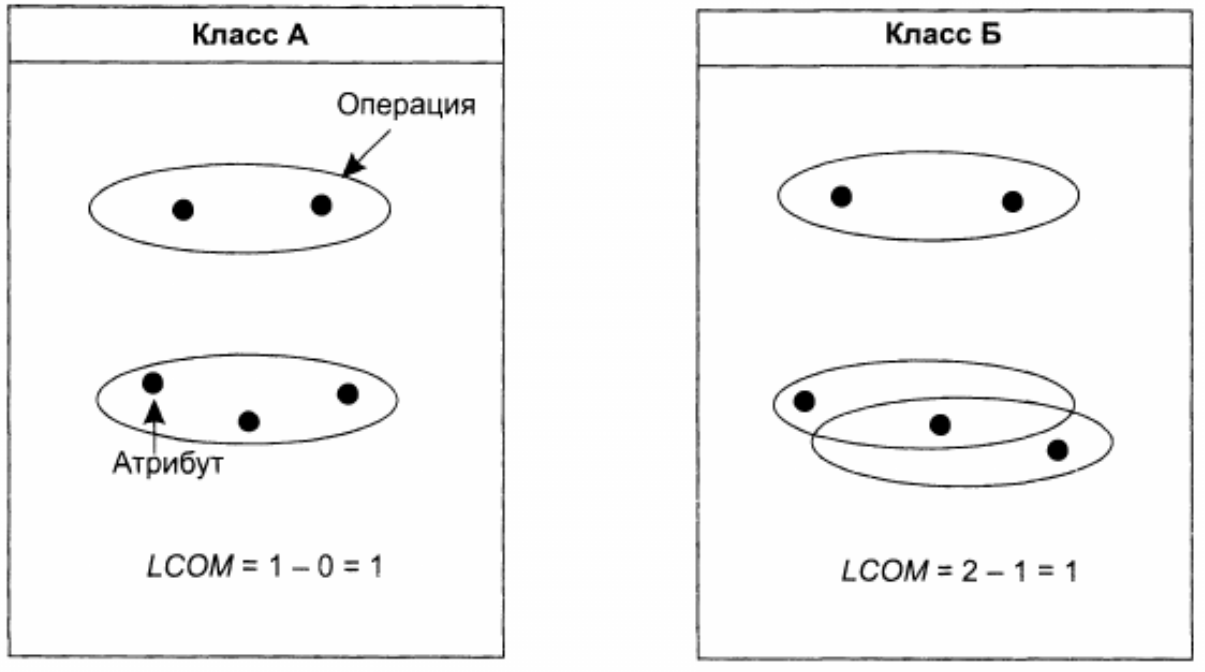
\includegraphics[width=0.7\textwidth]{lcomFail1.png}
        \end{center}
    \end{frame}

    \begin{frame}
        \frametitle{LCOM: недостатки (2)}
        \begin{center}
            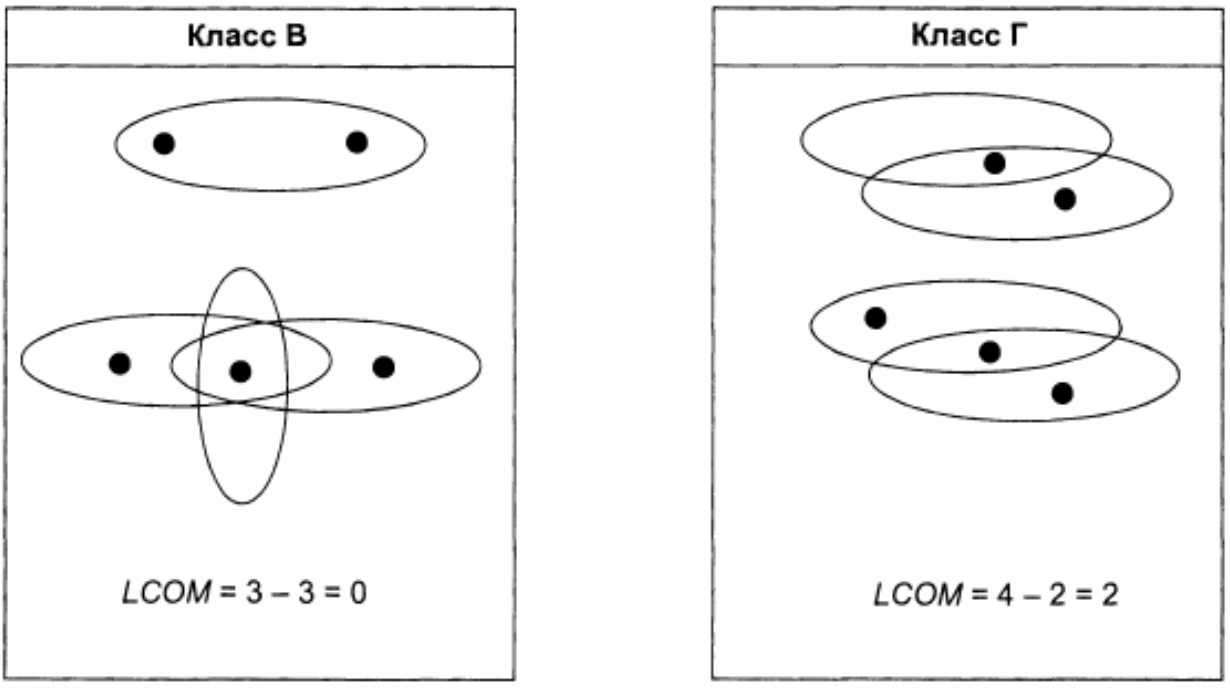
\includegraphics[width=0.7\textwidth]{lcomFail2.png}
        \end{center}
    \end{frame}

    \begin{frame}
        \frametitle{Модификация LCOM*}
        
        $$LCOM^* = \frac{\Biggl(\frac{1}{a}\sum\limits_{j=1}^{a}m(A_j)\Biggr) - m}{1 - m}$$

        \begin{itemize}
            \item $m$ --- количество методов класса
            \item $a$ --- количество атрибутов класса
            \item $m(A_j)$ --- количество методов, которые имеют доступ к атрибуту $A$
        \end{itemize}
    \end{frame}

    \begin{frame}
        \frametitle{Метрики Лоренца и Кидда}
        \begin{columns}
            \begin{column}{0.65\textwidth}
                \begin{itemize}
                    \item Метрики, ориентированные на классы
                    \begin{itemize}
                        \item Class Size (CS, <= 20)
                        \item Number of Operations Overridden by a Subclass (NOO, <= 3)
                        \item Number of Operations Added by a Subclass (NOA, <= 4)
                        \item Specialization Index (SI, <= 0.15)
                            $SI = (NOO \times \text{уровень}) / M_\text{общ.}$
                    \end{itemize}
                    \item Метрики, ориентированные на операции
                    \begin{itemize}
                        \item Average Operation Size ($OS_{avg}$, <=9)
                        \item Operation Complexity (OC)
                        \item Average Number of Parameters per operation ($NP_{avg}$)
                    \end{itemize}
                \end{itemize}
            \end{column}
            \begin{column}{0.35\textwidth}
                \begin{center}
                    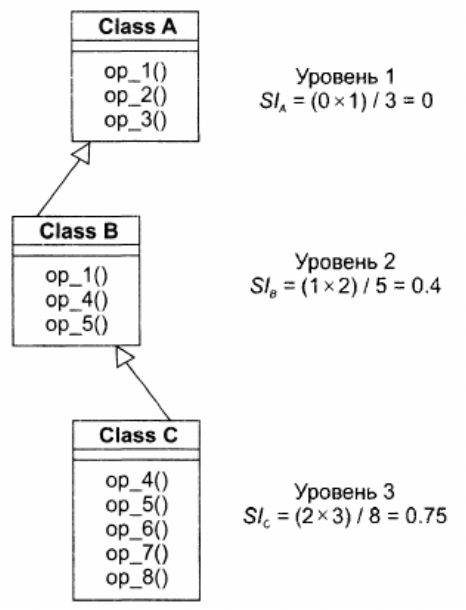
\includegraphics[width=\textwidth]{siCalculation.png}
                \end{center}
            \end{column}
        \end{columns}
    \end{frame}

    \begin{frame}
        \frametitle{Набор метрик Фернандо Абреу (MOOD)}
        \begin{itemize}
            \item Фактор закрытости метода (MHF)
            \item Фактор закрытости атрибута (AHF)
            \item Фактор наследования метода (MIF)
            \item Фактор наследования атрибута (AIF)
            \item Фактор полиморфизма (POF)
            \item Фактор сопряжения (СOF)
        \end{itemize}
    \end{frame}

    \begin{frame}
        \frametitle{Фактор закрытости метода (MHF)}
        $$MHF = \frac{\sum\limits_{i=1}^{TC}M_h(C_i)}{\sum\limits_{i=1}^{TC}M_a(C_i)}$$
        \begin{itemize}
            \item $M_h(C_i)$ --- количество private-методов в классе $C_i$
            \item $M_a(C_i)$ --- общее количество методов в классе $C_i$ (без унаследованных)
        \end{itemize}
    \end{frame}

    \begin{frame}
        \frametitle{Фактор закрытости свойства (AHF)}
        $$AHF = \frac{\sum\limits_{i=1}^{TC}A_h(C_i)}{\sum\limits_{i=1}^{TC}A_a(C_i)}$$
        \begin{itemize}
            \item $A_h(C_i)$ --- количество private-атрибутов в классе $C_i$
            \item $A_a(C_i)$ --- общее количество атрибутов в классе $C_i$
        \end{itemize}
    \end{frame}

    \begin{frame}
        \frametitle{Фактор наследования метода (MIF)}
        $$MIF = \frac{\sum\limits_{i=1}^{TC}M_i(C_i)}{\sum\limits_{i=1}^{TC}M_a(C_i)}$$
        \begin{itemize}
            \item $M_i(C_i)$ --- количество унаследованных и не переопределенных методов в классе $C_i$
            \item $M_a(C_i)$ --- общее количество методов в классе $C_i$
        \end{itemize}
    \end{frame}

    \begin{frame}
        \frametitle{Фактор наследования свойства (AIF)}
        $$AIF = \frac{\sum\limits_{i=1}^{TC}A_i(C_i)}{\sum\limits_{i=1}^{TC}A_a(C_i)}$$
        \begin{itemize}
            \item $A_i(C_i)$ --- количество унаследованных и не переопределенных атрибутов в классе $C_i$
            \item $A_a(C_i)$ --- общее количество атрибутов в классе $C_i$
        \end{itemize}
    \end{frame}

    \begin{frame}
        \frametitle{Фактор полиморфизма (POF)}
        $$POF = \frac{\sum\limits_{i=1}^{TC}M_o(C_i)}{\sum\limits_{i=1}^{TC}M_n(C_i) \times DC(C_i)}$$
        \begin{itemize}
            \item $M_o(C_i)$ --- количество унаследованных и переопределенных методов в $C_i$
            \item $M_n(C_i)$ --- количество новых (не унаследованных и переопределенных) методов в $C_i$
            \item $DC(C_i)$ --- количество потомков класса $C_i$
        \end{itemize}
    \end{frame}

    \begin{frame}
        \frametitle{Фактор сопряжения (COF)}
        $$COF = \frac{\sum\limits_{i=1}^{TC}\biggl(\sum\limits_{j=1}^{TC}is\_client(C_i, C_j)\biggl)}{TC^2 - TC}$$

        \begin{equation*}
            is\_client(C_c, C_s) = \begin{cases}
                1, & \text{если}\ C_c => C_s \cap C_c \neq C_s \\
                0, & \text{в противном случае}.
            \end{cases}
        \end{equation*}

        \begin{itemize}
            \item $C_c$ => $C_s$ --- класс-клиент содержит по меньшей мере одну не унаследованную ссылку на атрибут или метод класса-поставщика
        \end{itemize}
    \end{frame}

    \begin{frame}
        \frametitle{Метрики для тестирования}
        \begin{itemize}
            \item Недостаток связности в методах
            \item Процент публичных и защищенных методов
            \item Публичный доступ к атрибутам
            \item Количество корневых классов
            \item Количество детей, Высота дерева наследования
            \item Процентное количество не переопределенных запросов
            \item Процентное количество динамических запросов
            \item Скачок класса, Скачок системы
        \end{itemize}
    \end{frame}

    \begin{frame}
        \begin{center}
            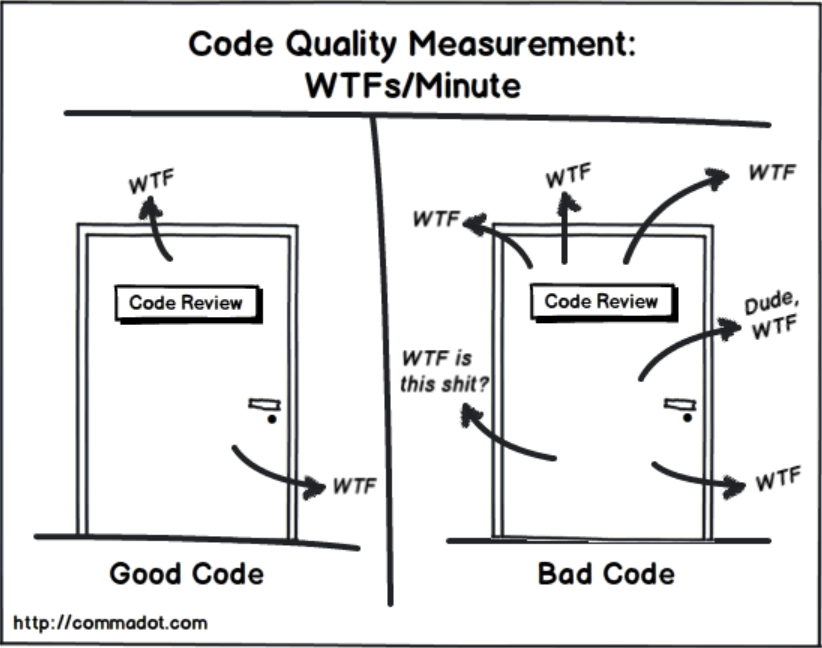
\includegraphics[width=0.7\textwidth]{wtfsPerMinute.png}
        \end{center}
    \end{frame}

    \begin{frame}
        \frametitle{Аудит программного кода}
        \begin{itemize}
            \item Сбор информации, накопление знаний, формирование эталонов
            \item Ручной
            \begin{itemize}
                \item Экспертный
                \item Расчётный
            \end{itemize}
            \item Автоматический
            \begin{itemize}
                \item \url{https://plugins.jetbrains.com/plugin/93-metricsreloaded}
                \item \url{http://metrics.sourceforge.net/}
                \item \url{https://www.codacy.com/}
            \end{itemize}
        \end{itemize}
    \end{frame}

    \section{CMM}

    \begin{frame}
        \frametitle{Capability Maturity Model Integration (CMMI)}
        \begin{itemize}
            \item Комплексная модель производительности и зрелости компании
            \item Пять уровней зрелости
            \item 22 области усовершенствования
            \begin{itemize}
                \item Управление процессами
                \item Управление проектами
                \item Инженерные области
                \item Служебные области
            \end{itemize}
            \item Цели: общие и специфические
            \item Best Practices
        \end{itemize}
    \end{frame}

    \begin{frame}
        \begin{center}
            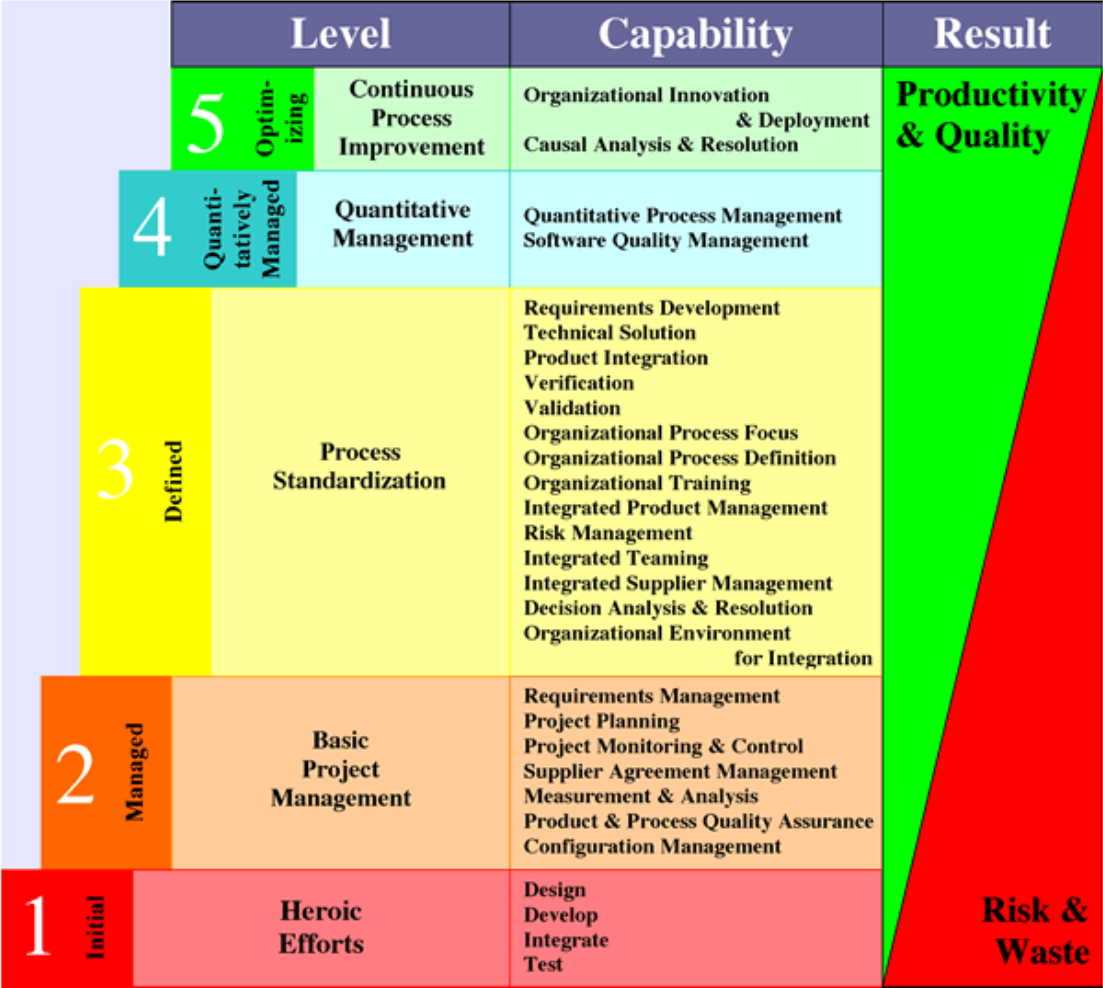
\includegraphics[height=0.95\textheight]{cmmi.png}
        \end{center}
    \end{frame}

    \section{Тестирование}

    \begin{frame}
        \frametitle{Тестирование}
        \begin{itemize}
            \item Любая программа содержит ошибки
            \item Если программа не содержит ошибок, их содержит алгоритм, который реализует эта программа
            \item Если ни программа, ни алгоритм ошибок не содержат, такая программа даром никому не нужна
        \end{itemize}
    \end{frame}

    \begin{frame}
        \frametitle{Виды тестирования}
        \begin{itemize}
            \item По объекту тестирования
            \begin{itemize}
                \item Функциональное
                \item Тестирование производительности
                \begin{itemize}
                    \item Нагрузочное
                    \item Стресс-тестирование
                    \item Тестирование стабильности
                \end{itemize}
                \item Тестирование удобства использования
                \item Тестирование интерфейса пользователя
                \item Тестирование безопасности
                \item Тестирование локализации
                \item Тестирование совместимости
            \end{itemize}
        \end{itemize}
    \end{frame}

    \begin{frame}
        \frametitle{Виды тестирования (2)}
        \begin{itemize}
            \item По знанию о системе
            \begin{itemize}
                \item White box
                \item Black box
            \end{itemize}
            \item По степени автоматизации
            \begin{itemize}
                \item Ручное
                \item Автоматическое
            \end{itemize}
            \item По степени подготовленности
            \begin{itemize}
                \item Тестирование по документации
                \item Ad-hoc тестирование
            \end{itemize}
        \end{itemize}
    \end{frame}

    \begin{frame}
        \frametitle{Виды тестирования (3)}
        \begin{itemize}
            \item По времени проведения
            \begin{itemize}
                \item Альфа-тестирование
                \begin{itemize}
                    \item Smoke testing
                    \item Тестирование новой функциональности
                    \item Регрессионное тестирование
                    \item Приемочное тестирование
                \end{itemize}
                \item Бета-тестирование
            \end{itemize}
            \item По степени изолированности компонентов
            \begin{itemize}
                \item Компонентное/модульное
                \item Интеграционное
                \item Системное
            \end{itemize}
        \end{itemize}
    \end{frame}

    \begin{frame}
        \frametitle{Почему тесты полезны}
        \begin{itemize}
            \item Помогают искать ошибки
            \item Облегчают изменение программы
            \begin{itemize}
                \item Помогают при рефакторинге
            \end{itemize}
            \item Тесты --- документация к коду
            \item Помогают улучшить архитектуру
            \begin{itemize}
                \item Приложение как набор библиотек
                \item Многоуровневая архитектура
                \item Управление зависимостями
                \begin{itemize}
                    \item Изоляция компонент
                    \item Dependency injection
                \end{itemize}
            \end{itemize}
        \end{itemize}
    \end{frame}

\end{document}